
%(BEGIN_QUESTION)
% Copyright 2006, Tony R. Kuphaldt, released under the Creative Commons Attribution License (v 1.0)
% This means you may do almost anything with this work of mine, so long as you give me proper credit

Det er ofte mulig å konfigurere en ventilposisjoner slik at virkningen til en reguleringsventil reverseres (signal-til-åpne eller signal-til-stenge). En grunn til å gjøre dette er å lage den ene halvdelen av et split-range-oppsett, der den andre ventilen virker motsatt (enten komplementært eller eksklusivt). Se på følgende reguleringsventil, der posisjoneren er konfigurert til å reagere ``revers'':

$$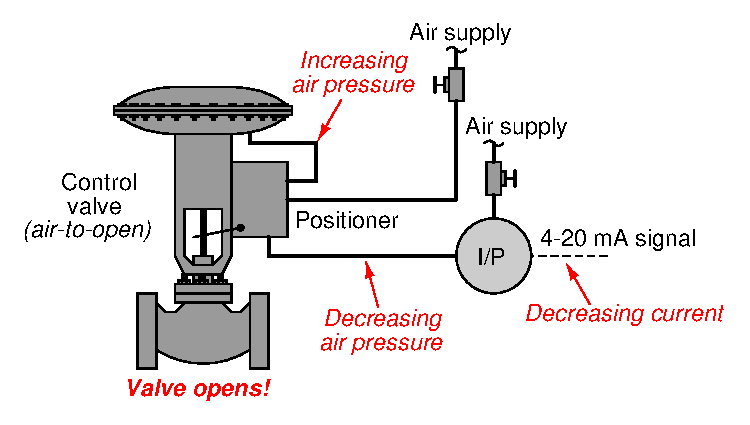
\includegraphics[width=15.5cm]{i01399x01.eps}$$

Selv om dette kan være mulig, er det kanskje ikke den beste løsningen sett fra et feilsikkert perspektiv. Forklar hvorfor ventilens feilsikre modus kan bli kompromittert med en slik kalibrering av posisjoneren. Forklar deretter hva som er den {\it beste} måten å reversere ventilvirkningen på.

\vskip 20pt \vbox{\hrule \hbox{\strut \vrule{} {\bf Forslag til sokratisk diskusjon} \vrule} \hrule}

\begin{itemize}
\item{} En kraftig problemløsningsteknikk er å utføre et {\it tankeeksperiment} der du mentalt simulerer hvordan et system responderer på et forestilt sett av betingelser. Beskriv et nyttig ``tankeeksperiment'' for dette systemet, og hvordan resultatene av dette tankeeksperimentet hjelper deg med å besvare spørsmålet.
\item{} Identifiser et praktisk reversvirkende område for en reguleringsventil, og en anvendelse der det kan brukes.
\end{itemize}

\underbar{file i01399}
%(END_QUESTION)





%(BEGIN_ANSWER)

Feilmodus for denne ventilen ved tap av forsyningsluft til posisjoneren vil ikke være den samme som feilmodus ved tap av lufttrykk fra I/P-enheten eller ved tap av likestrøm til I/P-enheten.
 
%(END_ANSWER)





%(BEGIN_NOTES)

Slik den er konfigurert i illustrasjonen:

\begin{itemize}
\item{} Bortfall av luftforsyning til posisjoneren = {\it ventilen stenger}
\item{} Bortfall av luftforsyning til I/P = {\it ventilen åpner}
\item{} Bortfall av strømsignal til I/P = {\it ventilen åpner}
\end{itemize}

\vskip 10pt

En bedre måte å reversere ventilresponsen på er å reversere aktuatoren og bruke direktevirkende posisjonerer, slik at ventilen endres fra luft-til-åpne til luft-til-stenge. Da blir feilmodusen konsekvent (ventilen stenger), uansett hvor lufttrykk (eller strømsignal) faller bort.

%INDEX% Final Control Elements, valve: positioner

%(END_NOTES)

